\documentclass[11pt,journal,transmag,final]{IEEEtran}

\usepackage{graphicx}
\usepackage{listings}
\usepackage{makecell}
\usepackage{hyperref}

\begin{document}

    \title{Collective Report B}
    \author{
        \IEEEauthorblockA{Daniel Carl Jones,}
        \IEEEauthorblockA{Department of Computer Science, University of Sheffield.}
        \IEEEauthorblockA{\today{}.}
    }

    \maketitle

    \section{Introduction}

    This report explores a problem involving reinforcement learning. The scenario includes a robot in two-dimensional space (a room) searching for a power source to recharge. Recharging is therefore its reward creating positive reinforcement.

    The programmes presenting the results are implemented in Python\footnote{https://www.python.org/}. They utilise two main libraries: NumPy\footnote{http://www.numpy.org/} is used for linear algebra and maths; MatPlotLib\footnote{https://matplotlib.org/} is used to create graphs and visualsations in order to demonstrate the results.

    The specifics of the problem are mostly left open. The following assumptions have been made.

    \begin{itemize}
        \item The space can have an arbitrary shape in two dimensions.
        \item The power source is in a fixed position and always available.
        \item Leaving the defined space is bad --- i.e. hitting the walls of the room. Therefore, hitting the wall should provide punishment or negative reinforcement.
        \item The robot can explore only a set amount of time before discharging completely.
        \item The robot can only observe its position in the room and the possible actions it can take. The reward location is not visible nor any information about positions not immediately accessible.
    \end{itemize}

    \section{Standard Solution with SARSA}
    \label{sec:standard-sarsa}

    A standard solution has been developed using the SARSA algorithm with Q-values. The space has been discretised into a 2D grid which is 4 units by 3 units.

    The robot is allocated a 'charge' (the maximum number of choices) with a value of the number of grid spaces raised to the power of $\frac{3}{2}$. A higher number than this meant that the simulation took a long period of time to run.

    The robot is allocated 25 episode to learn the environment and the figures in this report are reported accordingly. Hitting a wall gives a negative reward or punishment of value $-1$. Finding the charging source gives a reward of $+1$.

    A few classes have been developed in code listing \ref{lst:classes} to assist with the algorithm. The SARSA homing algorithm implementation is shown in listing \ref{lst:sarsa}

    Each individual run of the algorithm will produce a different result. This is because the agent begins with no prior knowledge of the estimated reward at a state for some action --- all estimated rewards are initialised at 0. Hence, the agent must \textbf{explore} before it can begin to \textbf{exploit} its knowledge of the environment. This random exploration can cause the agent to stumble on the reward very quickly or slowly depending on the initial direction it took, especially when working in more than one dimension.

    The initial results are shown in figures \ref{fig:standard-sarsa:mean-reward} and \ref{fig:standard-sarsa:mean-steps}. Figure \ref{fig:standard-sarsa:mean-reward} shows the reward averaged over 250 repetitions compared to the episode number. Figure \ref{fig:standard-sarsa:mean-steps} shows the steps required to reach a terminal state averaged over 250 repetitions compared to the episode number.

    \begin{figure}
        \begin{center}
            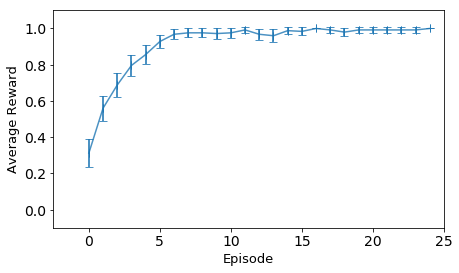
\includegraphics[width=\linewidth,keepaspectratio]{figures/ss-mean-reward.png}
            \caption{Mean Reward over Episodes}
            \label{fig:standard-sarsa:mean-reward}
        \end{center}
    \end{figure}

    \begin{figure}
        \begin{center}
            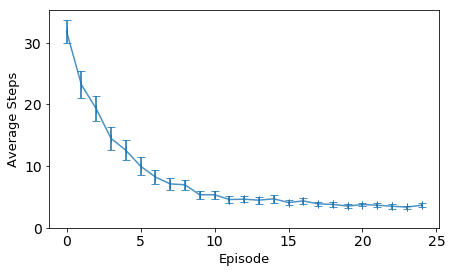
\includegraphics[width=\linewidth,keepaspectratio]{figures/ss-mean-steps.png}
            \caption{Mean Steps over Episodes}
            \label{fig:standard-sarsa:mean-steps}
        \end{center}
    \end{figure}

    \section{Optimal Learning Rate, Discount Factor, and Epsilon Probability}

    There are numerous parameters to tweak when modelling this scenario. Most notable are the learning rate $\eta$, the discount factor $\gamma$, and the probability of exploration $\epsilon$.

    The results in section \ref{sec:standard-sarsa} were based on using the following parameters: $\eta = 0.9$, $\gamma = 0.9$, and $\epsilon = 0.1$.

    In order to compare different parameter values, a good performance metric should be used. A few were considered: MacGlashan of Cogitai highlights the culmulative reward as a good performance measure, plotting this against the episode number \cite{LearningPerformance}. However, it didn't really show much information with this problem. Instead, this report simply uses the average steps versus the episode number. The camparisons can be shown in figure \ref{fig:varying-params:comparison}. The code for running all these variations is shown in listing \ref{lst:experiments}.

    \begin{figure}
        \begin{center}
            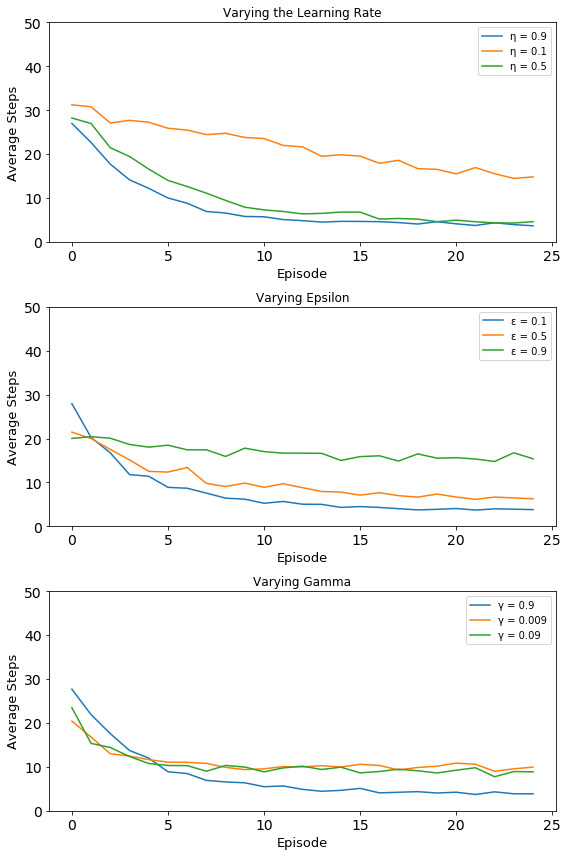
\includegraphics[width=\linewidth,keepaspectratio]{figures/varying-parameters.png}
            \caption{Varying $\eta$, $\gamma$, and $\epsilon$}
            \label{fig:varying-params:comparison}
        \end{center}
    \end{figure}

    In the comparison between three learning rate values, $\eta = 0.9$ seems optimal. A large detriment in performance can be seen with a learning rate as low as 0.1.

    When varying epsilon, the parameter indicating the probability of exploration, large values initially show better results but the performance does not improve with the number of episodes and a value of $\epsilon = 0.1$ quickly shows itself as the most optimal requiring approximately 5 steps to reach the goal. This is unlike $\epsilon = 0.9$ which requires around 18 steps. This makes sense --- once the agent has learnt more about the environment it should be trusting what it has discovered.

    The last graph compares different values for the discount rate gamma. There is not a great deal in variation of performance but a high value proves to be the best in the long run. $\gamma = 0.9$ proves to be best beyond episode 5 consistently finding the goal within approximately 5 steps.

    Without further comparing how each parameter's performance changes while varying another parameter, values of $\eta = 0.9$, $\gamma = 0.9$, and $\epsilon = 0.1$ seem optimal. Of course, it may be found that the parameters have different relationships together and different combinations of values may work better.

    \section{Visualising The Weights}

    The approach used in this report to visualise the weights is to convert each weight value into a vector with an x and y co-ordinate. For example, the \textit{North} action may have a Q value of $0.2$. This would he multiplied by the vector $(0, 1)$ to produce $(0, 0.2)$. The mean can be taken of each of these vectors produced from the actions, and this new direction vector can then be plotted on to the grid. The standard SARSA implementation's weights are plotted in figure \ref{fig:visualising-weights:plot}. A common name for this type of plot is a 'Quiver' or 'Velocity' plot.

    \begin{figure}
        \begin{center}
            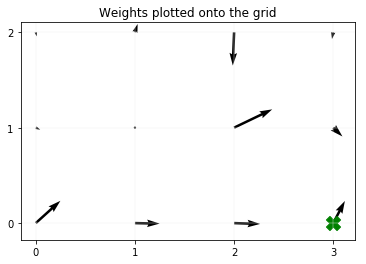
\includegraphics[width=\linewidth,keepaspectratio]{figures/ss-qvalues.png}
            \caption{Visualisation of Weights}
            \label{fig:visualising-weights:plot}
        \end{center}
    \end{figure}

    The plot does not appear to show outstanding results, however it is possible to see a general direction in most segments towards the charging point shown by the green cross.

    \section{Increasing Quantity of Actions}

    The standard implementation in the previous sections has used four actions: North, East, South, and West. Increasing the action count to 8, we add North East, South East, and so on.

    Overall, it didn't seem to have a large affect on the model other than an increased computation time. The average reward and steps are plotted in figures \ref{fig:8-actions:mean-reward} and \ref{fig:8-actions:mean-steps} respectively, which can be compared to figures \ref{fig:standard-sarsa:mean-reward} and \ref{fig:standard-sarsa:mean-steps} in section \ref{sec:standard-sarsa}.

    \begin{figure}
        \begin{center}
            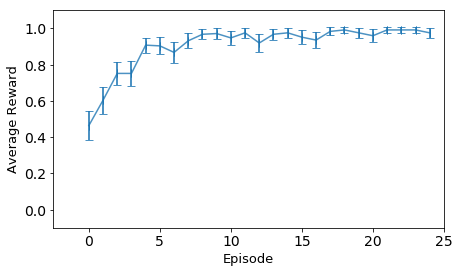
\includegraphics[width=\linewidth,keepaspectratio]{figures/8-mean-reward.png}
            \caption{Mean reward over episodes with 8 actions}
            \label{fig:8-actions:mean-reward}
        \end{center}
    \end{figure}

    \begin{figure}
        \begin{center}
            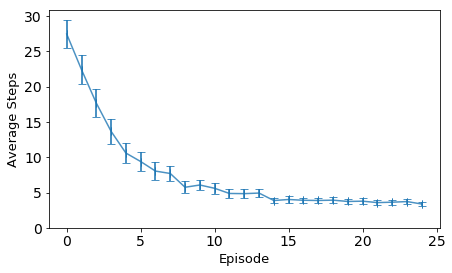
\includegraphics[width=\linewidth,keepaspectratio]{figures/8-mean-steps.png}
            \caption{Mean steps over episodes with 8 actions}
            \label{fig:8-actions:mean-steps}
        \end{center}
    \end{figure}

    \section{Reproducing The Results}

    The code used to produce these results are included as a Jupyter Notebook\footnote{http://jupyter.org/}. The graphs and results are taken directly from the output of the project.

    If using an environment like Anaconda, the libraries should all be preinstalled and require no setup. Starting up a Jupyter server for the notebooks should be all that is required.
    \begin{appendices}
        \section{Assignment Completion}

        Most of the points indicated in the assignment brief have been completed excluding the comparison of SARSA and Q-learning due to time constraints.


        \onecolumn
        \section{Code Listings}

        This section contains simplified code listings for both algorithms. For full solutions, see the seperated Jupyter notebooks.

        \begin{lstlisting}[language=Python, caption=Classes, basicstyle=\footnotesize, label=lst:classes]
###
### Object Definitions
###

class Grid():
    def __init__(self, shape, terminal_positions = [], rewards=[]):
        self.grid = np.zeros(shape)
        self.terminal_positions = terminal_positions
        self.rewards = rewards
        
    def random_position(self):
        return (
            np.random.randint(self.get_shape()[0]),
            np.random.randint(self.get_shape()[1])
        )
    
    def get_shape(self):
        return self.grid.shape
    
    def get_size(self):
        max_x, max_y = self.get_shape()
        return max_x * max_y
    
    def is_terminal(self, position):
        return position in self.terminal_positions
    
    def as_vector(self, position):
        x, y = position
        v = np.zeros(self.get_shape())
        v[x,y] = 1
        return v.reshape(self.get_size(), 1)
    
    def get_possible_actions(self, position):
        possible_actions = [e for e in Action]
        x, y = position
        
        if y >= self.get_shape()[1] - 1:
            if (Action.NORTH in possible_actions):
                possible_actions.remove(Action.NORTH)
            if (Action.NORTH_WEST in possible_actions):
                possible_actions.remove(Action.NORTH_WEST)
            if (Action.NORTH_EAST in possible_actions):
                possible_actions.remove(Action.NORTH_EAST)
        if x >= self.get_shape()[0] - 1:
            if (Action.EAST in possible_actions):
                possible_actions.remove(Action.EAST)
            if (Action.NORTH_EAST in possible_actions):
                possible_actions.remove(Action.NORTH_EAST)
            if (Action.SOUTH_EAST in possible_actions):
                possible_actions.remove(Action.SOUTH_EAST)
        if y < 1:
            if (Action.SOUTH in possible_actions):
                possible_actions.remove(Action.SOUTH)
            if (Action.SOUTH_EAST in possible_actions):
                possible_actions.remove(Action.SOUTH_EAST)
            if (Action.SOUTH_WEST in possible_actions):
                possible_actions.remove(Action.SOUTH_WEST)
        if x < 1:
            if (Action.WEST in possible_actions):
                possible_actions.remove(Action.WEST)
            if (Action.NORTH_WEST in possible_actions):
                possible_actions.remove(Action.NORTH_WEST)
            if (Action.SOUTH_WEST in possible_actions):
                possible_actions.remove(Action.SOUTH_WEST)
            
        return possible_actions
    
    def __new_position_after_action(self, position, action):
        x, y = position
        if action in self.get_possible_actions(position):
            if action.vaguely(Action.NORTH):
                y += 1
            if action.vaguely(Action.EAST):
                x += 1
            if action.vaguely(Action.SOUTH):
                y -= 1
            if action.vaguely(Action.WEST):
                x -= 1
        return (x, y)
    
    def __reward_after_action(self, position, action):
        x, y = position
        if y >= self.get_shape()[1] and action.vaguely(Action.NORTH):
            return -1
        if x >= self.get_shape()[0] and action.vaguely(Action.EAST):
            return -1
        if y <= 0 and action.vaguely(Action.SOUTH):
            return -1
        if x <= 0 and action.vaguely(Action.WEST):
            return -1
        
        for reward_segment in self.rewards:
            loc, reward = reward_segment
            if self.__new_position_after_action(position, action) == loc:
                return reward
        
        return 0
    
    def perform(self, position, action):
        return (
            self.__new_position_after_action(position, action),
            self.__reward_after_action(position, action)
        )

class SarsaEnum(Enum):
    def _generate_next_value_(name, start, count, last_values):
        return count
    
@unique
class Action(SarsaEnum):
    NORTH = auto()
    NORTH_EAST = auto()
    EAST = auto()
    SOUTH_EAST = auto()
    SOUTH = auto()
    SOUTH_WEST = auto()
    WEST = auto()
    NORTH_WEST = auto()
    
    @classmethod
    def rand(cls):
        return cls(np.random.randint(len(cls)))
    
    def vaguely(self, action_to_compare):
        if action_to_compare == Action.NORTH:
            return self in [Action.NORTH, Action.NORTH_WEST, Action.NORTH_EAST]
        if action_to_compare == Action.EAST:
            return self in [Action.EAST, Action.NORTH_EAST, Action.SOUTH_EAST]
        if action_to_compare == Action.SOUTH:
            return self in [Action.SOUTH, Action.SOUTH_EAST, Action.SOUTH_WEST]
        if action_to_compare == Action.WEST:
            return self in [Action.WEST, Action.NORTH_WEST, Action.SOUTH_WEST]
        raise 'Action not recognised as main direction'
    
    def as_vector(self):
        v = np.zeros((len(type(self)), 1))
        v[self.value] = 1

        return v
        \end{lstlisting}

        \begin{lstlisting}[language=Python, caption=SARSA Algorithm Implementation, basicstyle=\footnotesize, label=lst:sarsa]
###
### Homing Algorithm / SARSA Implementation
###

grid_shape = (4,3)
charging_point = (3,0)

def sarsa_homing_nn(n_episodes, learning_rate, epsilon, gamma):
    
    grid = Grid(grid_shape, terminal_positions = [charging_point], rewards=[(charging_point, 1)])
    max_choices = math.ceil(grid.get_size() ** 1.5)

    # Initialise weights randomly. Connects input neurons (state) to output neurons (actions).
    # Weight is Q values.
    weights = np.random.rand(len(Action), grid.get_size())

    # Define info vectors (one position for each trial) and initialise it to zero
    r_history = np.zeros((1, n_episodes))
    steps_req_history = np.zeros((1, n_episodes))

    # Start the episode
    for episode in range(n_episodes):
        state = grid.random_position() # Initial state

        # Define and initialise at every episode the variables needed for SARSA
        input_v = np.zeros((grid.get_size(),1))
        output_v = np.zeros((len(Action),1))
        q_value = 0
        reward = 0
        steps_required = 0

        # Simulate the steps in the episode
        for step in range(max_choices):
            steps_required += 1
            input_v_ = grid.as_vector(state)
            
            # Compute state_q_values.  q_value = logsig(weights*input).
            # q_value is 2x1, one value for each output neuron
            state_q_values = (1 / (1 + np.exp(-1 * weights.dot(input_v_)))).flatten()
            
            winning_actions = np.argwhere(state_q_values == np.max(state_q_values)).flatten()

            # Implement the policy
            explore = np.random.rand() < epsilon
            if explore:
                possible_actions = grid.get_possible_actions(state)
                action = np.random.choice(possible_actions)
            else:
                random_winner = np.random.choice(winning_actions)
                action = Action(random_winner)

            state, reward_ = grid.perform(state, action)
            output_v_ = action.as_vector() # Update weights only for action selected.
            
            
            # Update weights
            q_value_ = state_q_values[action.value]
            d_w = learning_rate * (reward - (q_value - (gamma * q_value_)))
                * output_v.dot(input_v.T)
            weights += d_w

            # Update variables for sarsa
            q_value = q_value_
            output_v = output_v_
            input_v = input_v_
            reward = reward_
            
            if grid.is_terminal(state):
                break
            

        # Update weights for the terminal state
        d_w = learning_rate * (reward - q_value) * output_v.dot(input_v.T)
        weights += d_w

        # Store info for the current episode
        r_history[0,episode] = reward
        steps_req_history[0,episode] = steps_required

    return (r_history, steps_req_history, weights)
        \end{lstlisting}

        \begin{lstlisting}[language=Python, caption=Running Several Experiments, basicstyle=\footnotesize, label=lst:experiments]
        ###
        ### Parameter Setup
        ###
        
        n_episodes = 25    # int > 0
        learning_rates = [0.9, 0.1, 0.5] # real > 0
        epsilons = [0.1, 0.5, 0.9]    # real >= 0; epsilon=0 Greedy, otherwise epsilon-Greedy
        gammas = [0.9, 0.009, 0.09]         # 0 <= real <= 1
        repetitions = 250   # int > 0
        
        ###
        ### Experiments
        ###
        
        max_x, max_y = grid_shape
        weight_shape = (len(Action), max_x*max_y)
        
        lr_rewards = []
        lr_steps = []
        lr_weights = []
        
        for lr in log_progress(learning_rates, name='Learning Rates'):
            rewards = np.zeros((repetitions, n_episodes)) 
            steps_until_terminate = np.zeros((repetitions, n_episodes))
            weight_m = np.zeros((repetitions, *weight_shape))
        
            # Start iterations over episodes
            for j in log_progress(range(repetitions), name="Repetitions"):
                rewards[j,:], steps_until_terminate[j,:], weight_m[j,:] =
                    sarsa_homing_nn(n_episodes, lr, epsilons[0], gammas[0])
            
            lr_rewards.append(rewards)
            lr_steps.append(steps_until_terminate)
            lr_weights.append(weight_m)
            
        ep_rewards = []
        ep_steps = []
        ep_weights = []
        
        for ep in log_progress(epsilons, name='Epsilons'):
            rewards = np.zeros((repetitions, n_episodes))
            steps_until_terminate = np.zeros((repetitions, n_episodes))
            weight_m = np.zeros((repetitions, *weight_shape))
        
            # Start iterations over episodes
            for j in log_progress(range(repetitions), name="Repetitions"):
                rewards[j,:], steps_until_terminate[j,:], weight_m[j,:] =
                    sarsa_homing_nn(n_episodes, learning_rates[0], ep, gammas[0])
            
            ep_rewards.append(rewards)
            ep_steps.append(steps_until_terminate)
            ep_weights.append(weight_m)
            
        ga_rewards = []
        ga_steps = []
        ga_weights = []
        
        for ga in log_progress(gammas, name='Discount Rates'):
            rewards = np.zeros((repetitions, n_episodes))
            steps_until_terminate = np.zeros((repetitions, n_episodes))
            weight_m = np.zeros((repetitions, *weight_shape))
        
            # Start iterations over episodes
            for j in log_progress(range(repetitions), name="Repetitions"):
                rewards[j,:], steps_until_terminate[j,:], weight_m[j,:] =
                    sarsa_homing_nn(n_episodes, learning_rates[0], epsilons[0], ga)
            
            ga_rewards.append(rewards)
            ga_steps.append(steps_until_terminate)
            ga_weights.append(weight_m)
        \end{lstlisting}
    \end{appendices}

    \bibliography{assignment} 
    \bibliographystyle{IEEEtran}
\end{document}
